\let\negmedspace\undefined
\let\negthickspace\undefined
%\RequirePackage{amsmath}
\documentclass[journal,12pt,twocolumn]{IEEEtran}
 \usepackage[utf8]{inputenc}
 \usepackage{graphicx}
 \usepackage{amsmath}
 \usepackage{amsfonts}
 \usepackage{amssymb}
 \usepackage{enumitem}
\usepackage{mathtools}
\usepackage[breaklinks=false]{hyperref}
\usepackage{listings}
\usepackage{calc}

\newcommand{\BEQA}{\begin{eqnarray}}
\newcommand{\EEQA}{\end{eqnarray}}
\newcommand{\define}{\stackrel{\triangle}{=}}
\bibliographystyle{IEEEtran}
%\bibliographystyle{ieeetr}

\let\vec\mathbf

\providecommand{\abs}[1]{\left\vert#1\right\vert}
\providecommand{\res}[1]{\Res\displaylimits_{#1}}
\newcommand{\myvec}[1]{\ensuremath{\begin{pmatrix}#1\end{pmatrix}}}
\newcommand{\mydet}[1]{\ensuremath{\begin{vmatrix}#1\end{vmatrix}}}

\newcommand{\question}{\noindent \textbf{Question: }}
\newcommand{\solution}{\noindent \textbf{Solution: }}

\vspace{3cm}

\title{Assignment 1}
\author{Vishal Vijay Devadiga (CS21BTECH11061)}
\date{}
\begin{document}
% make the title area
\maketitle
\question
\begin{enumerate}[label=]
\item A(-1, 3), B(4,2) and C(3,-2) are the vertices of a triangle.
\begin{enumerate}
    \item Find the coordinates of the centroid G of the triangle
    \item Find the equation of the line through G and parallel to AC.
\end{enumerate}
\end{enumerate}
\solution
\begin{enumerate}
	\begin{figure}[htbp]
	\centerline{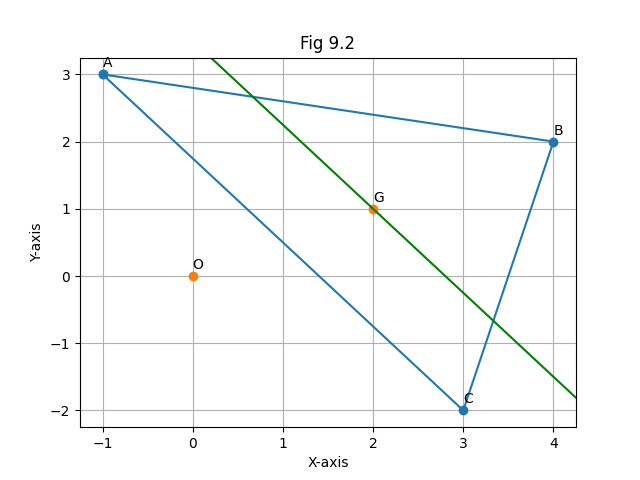
\includegraphics[scale = 0.6]{./figs/9.2.png}}
	\label{Figure 9.2}
	\end{figure}
\item Let $\vec{A}, \vec{B}, \vec{C}$ be the points vectors OA,OB,OC respectively, where O is the origin.
	Thus,
	\begin{align}
		\vec{A} = \myvec{-1 \\ 3} ,
		\vec{B} = \myvec{4 \\ 2}  ,
		\vec{C} = \myvec{3 \\ -2}
	\end{align}
	Using centroid formula,
    the desired point vector $\vec{G}$ is given by:
    \begin{align}
        \vec{G}&= \frac{1}{3}(\vec{A} + \vec{B} + \vec{C})
        \\
        &= \frac{1}{3}(\myvec{-1 \\ 3} + \myvec{4 \\ 2} + \myvec{3 \\ -2})
        \\
        &=\frac{1}{3}\myvec{6 \\ 3}
        \\
        &= \myvec{2 \\ 1}
    \end{align}
    $\vec{G}$ is the point vector $\myvec{2 \\ 1}$
\item Let L be the line that passes through G such that $L \parallel AC$
    Then, L can be expressed as $\vec{G} + k\hat{AC}$
    \begin{align}
        \hat{AC} &= \frac{\vec{C} - \vec{A}}{\abs{\vec{C} - \vec{A}}}
		\\        
        &= \frac{\myvec{3 \\ -2} - \myvec{-1 \\ 3}}{\abs{\myvec{3 \\ -2} - \myvec{-1 \\ 3}}}
        \\
        &= \frac{\myvec{4 \\ -5}}{\abs{\myvec{4 \\ -5}}}
		\\        
        &= \frac{\myvec{4 \\ -5}}{\sqrt{41}}
        \\
        L &= \myvec{2 \\ 1} + \frac{k}{\sqrt{41}}\myvec{4 \\ -5}
    \end{align}
    Thus, Line L is $\myvec{2 \\ 1} + m\myvec{4 \\ -5}$
\end{enumerate}
\end{document} 
